\documentclass[fleqn,10pt]{wlscirep}
\title{Git for Science}

\author[1,*]{Adam Steer}
\author[2]{Oliver Clements}
\author[2]{Julia Wagemann}
\author[3]{Carsten Ehbrecht}

\affil[1]{NCI, Australia}
\affil[2]{PML, UK}
\affil[3]{DKRZ, Germany}


\keywords{Git, LaTeX, Overleaf, EGU}

\begin{abstract}
  A workshop about how to use git for managing science tasks.
  Or \emph{how to spend less time hunting for the last working version; and keep track of collaborative works}.
\end{abstract}
\begin{document}

\flushbottom
\maketitle

\thispagestyle{empty}

\section*{Warm up}

How do you write your papers ... which tools are you using? Any experience with Git or other version control systems?

\section*{Getting Started}

Get used to Git. Try the basic commands.

\section*{Let us work on an example}

Work on an Overleaf document:

\begin{itemize}
  \item Edit it online.
  \item Share it with other people and work on it at the same time.
  \item Work on this Overleaf document offline using the Overleaf git repo.
  \item Share your local git repo with others and work togther on it.
  \item Try to create a conflict and solve it.
\end{itemize}

A conflict shown in the terminal.
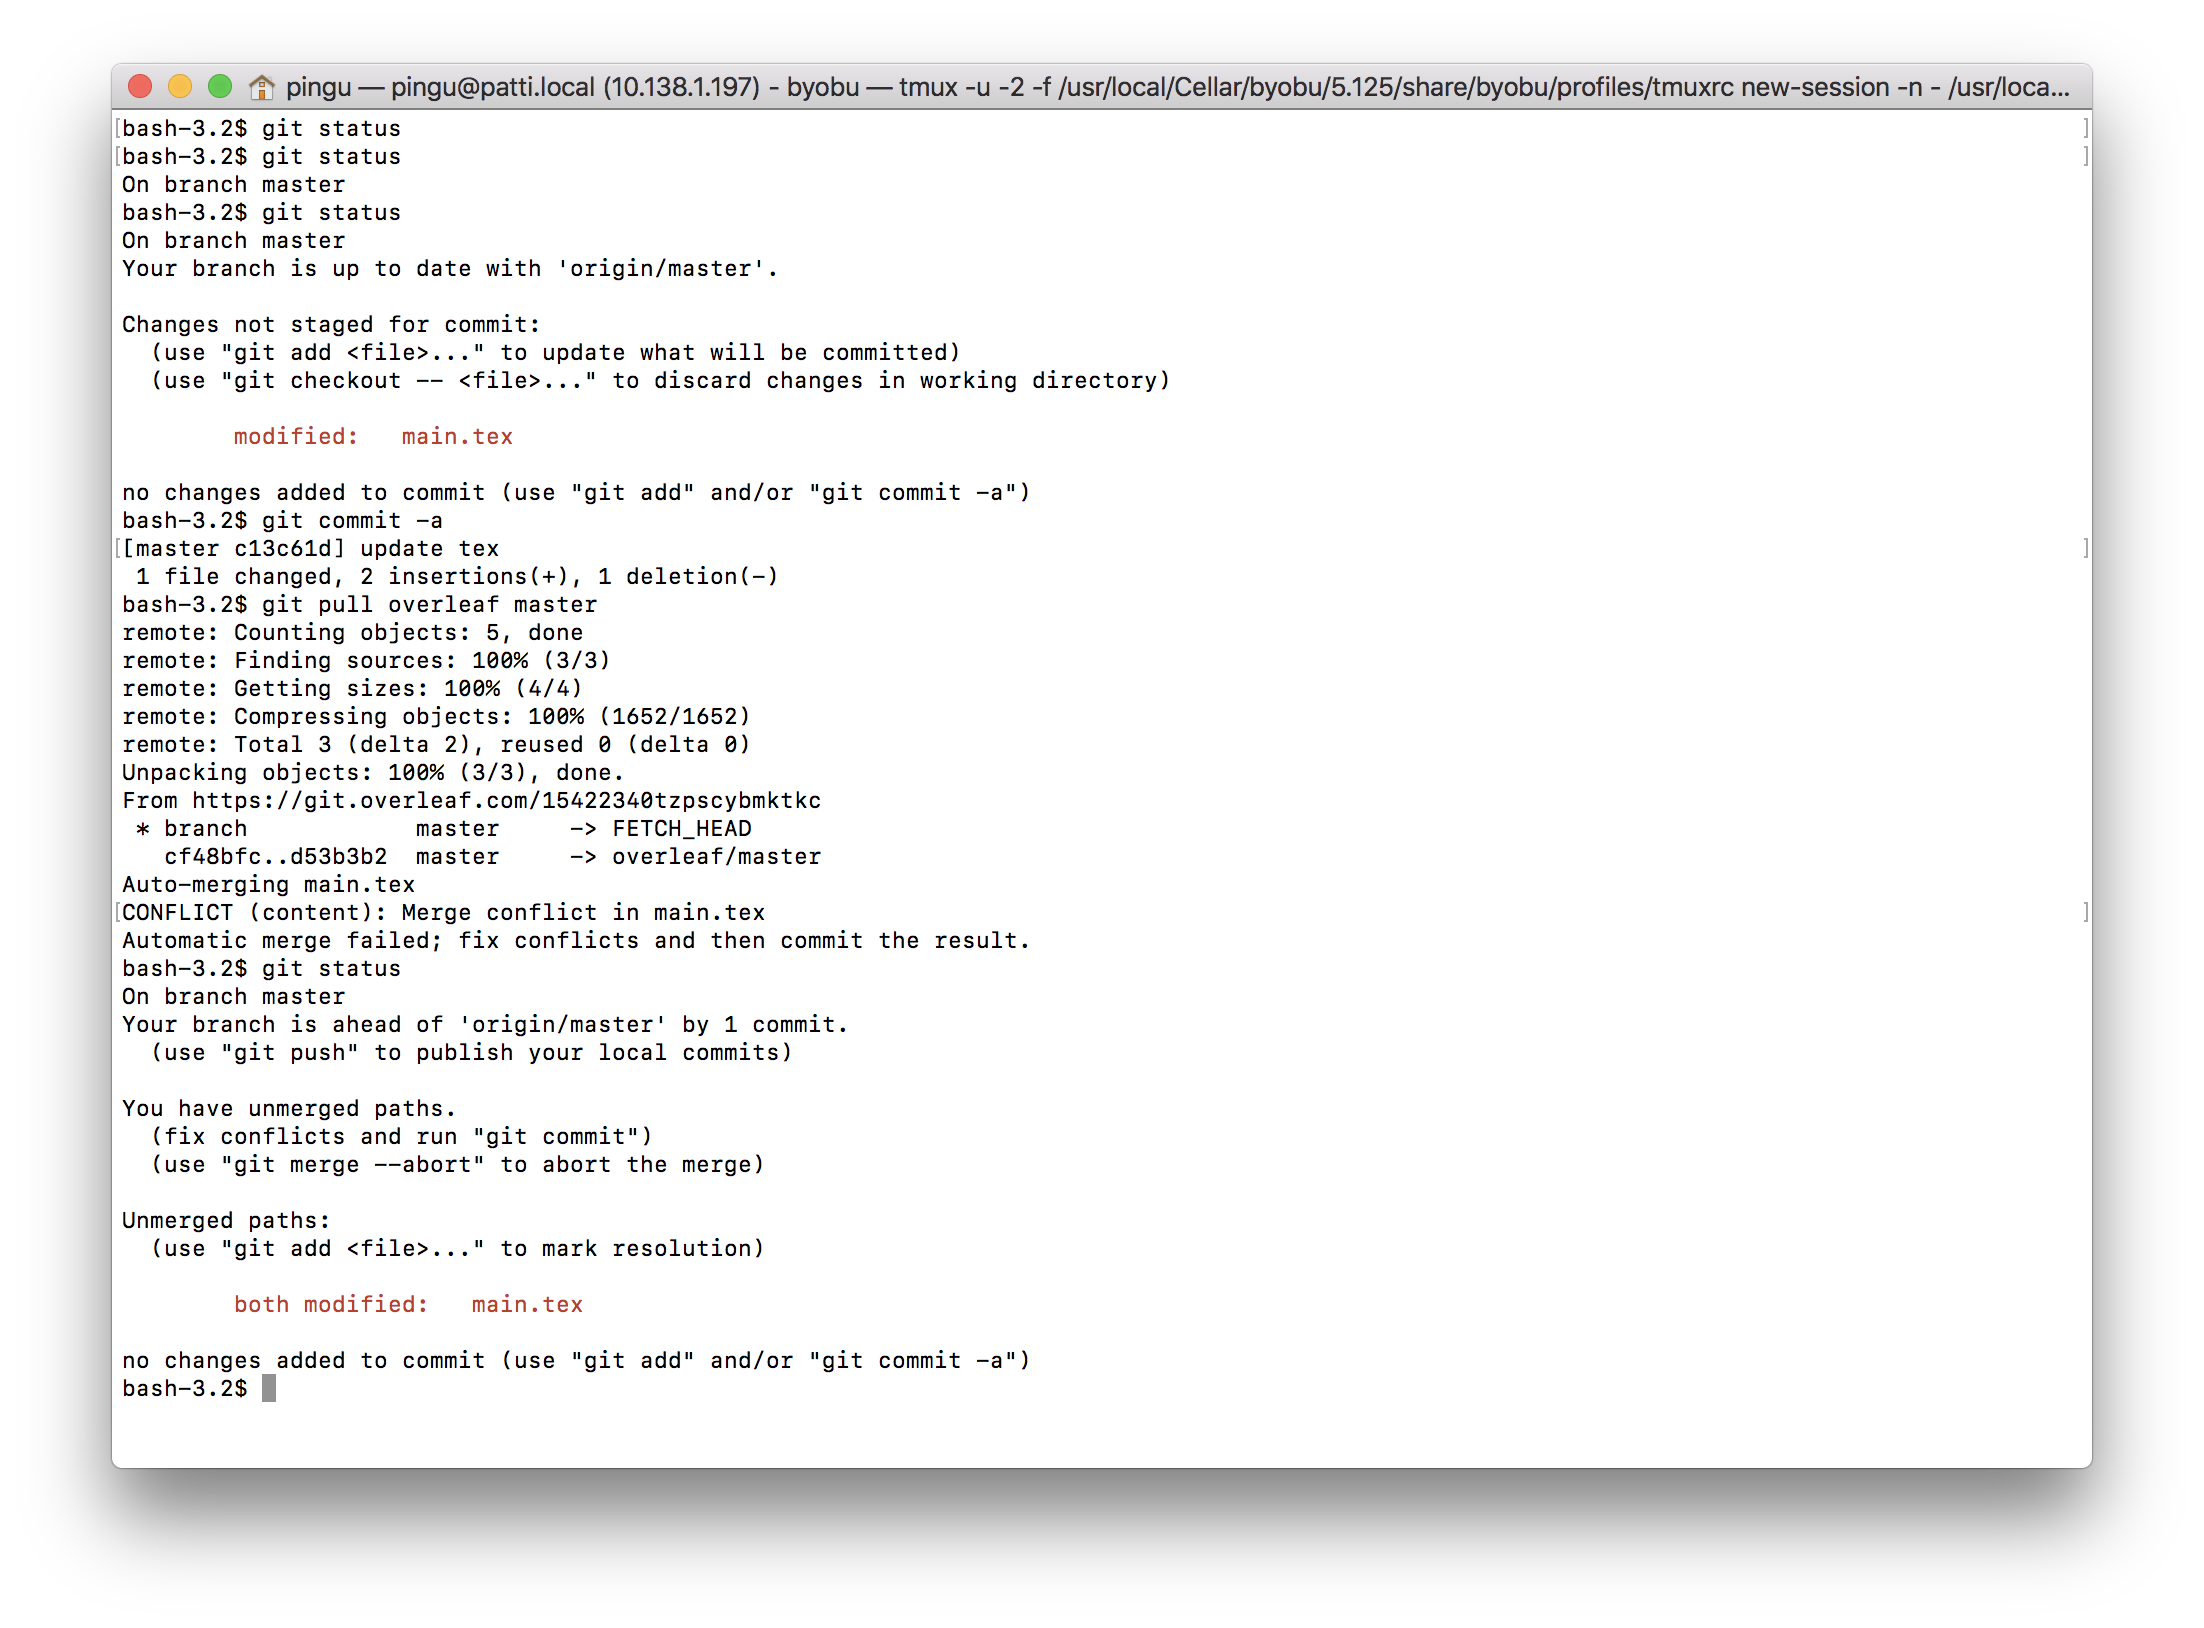
\includegraphics[width=20em]{terminal-conflict}

A conflict shown in Atom editor.
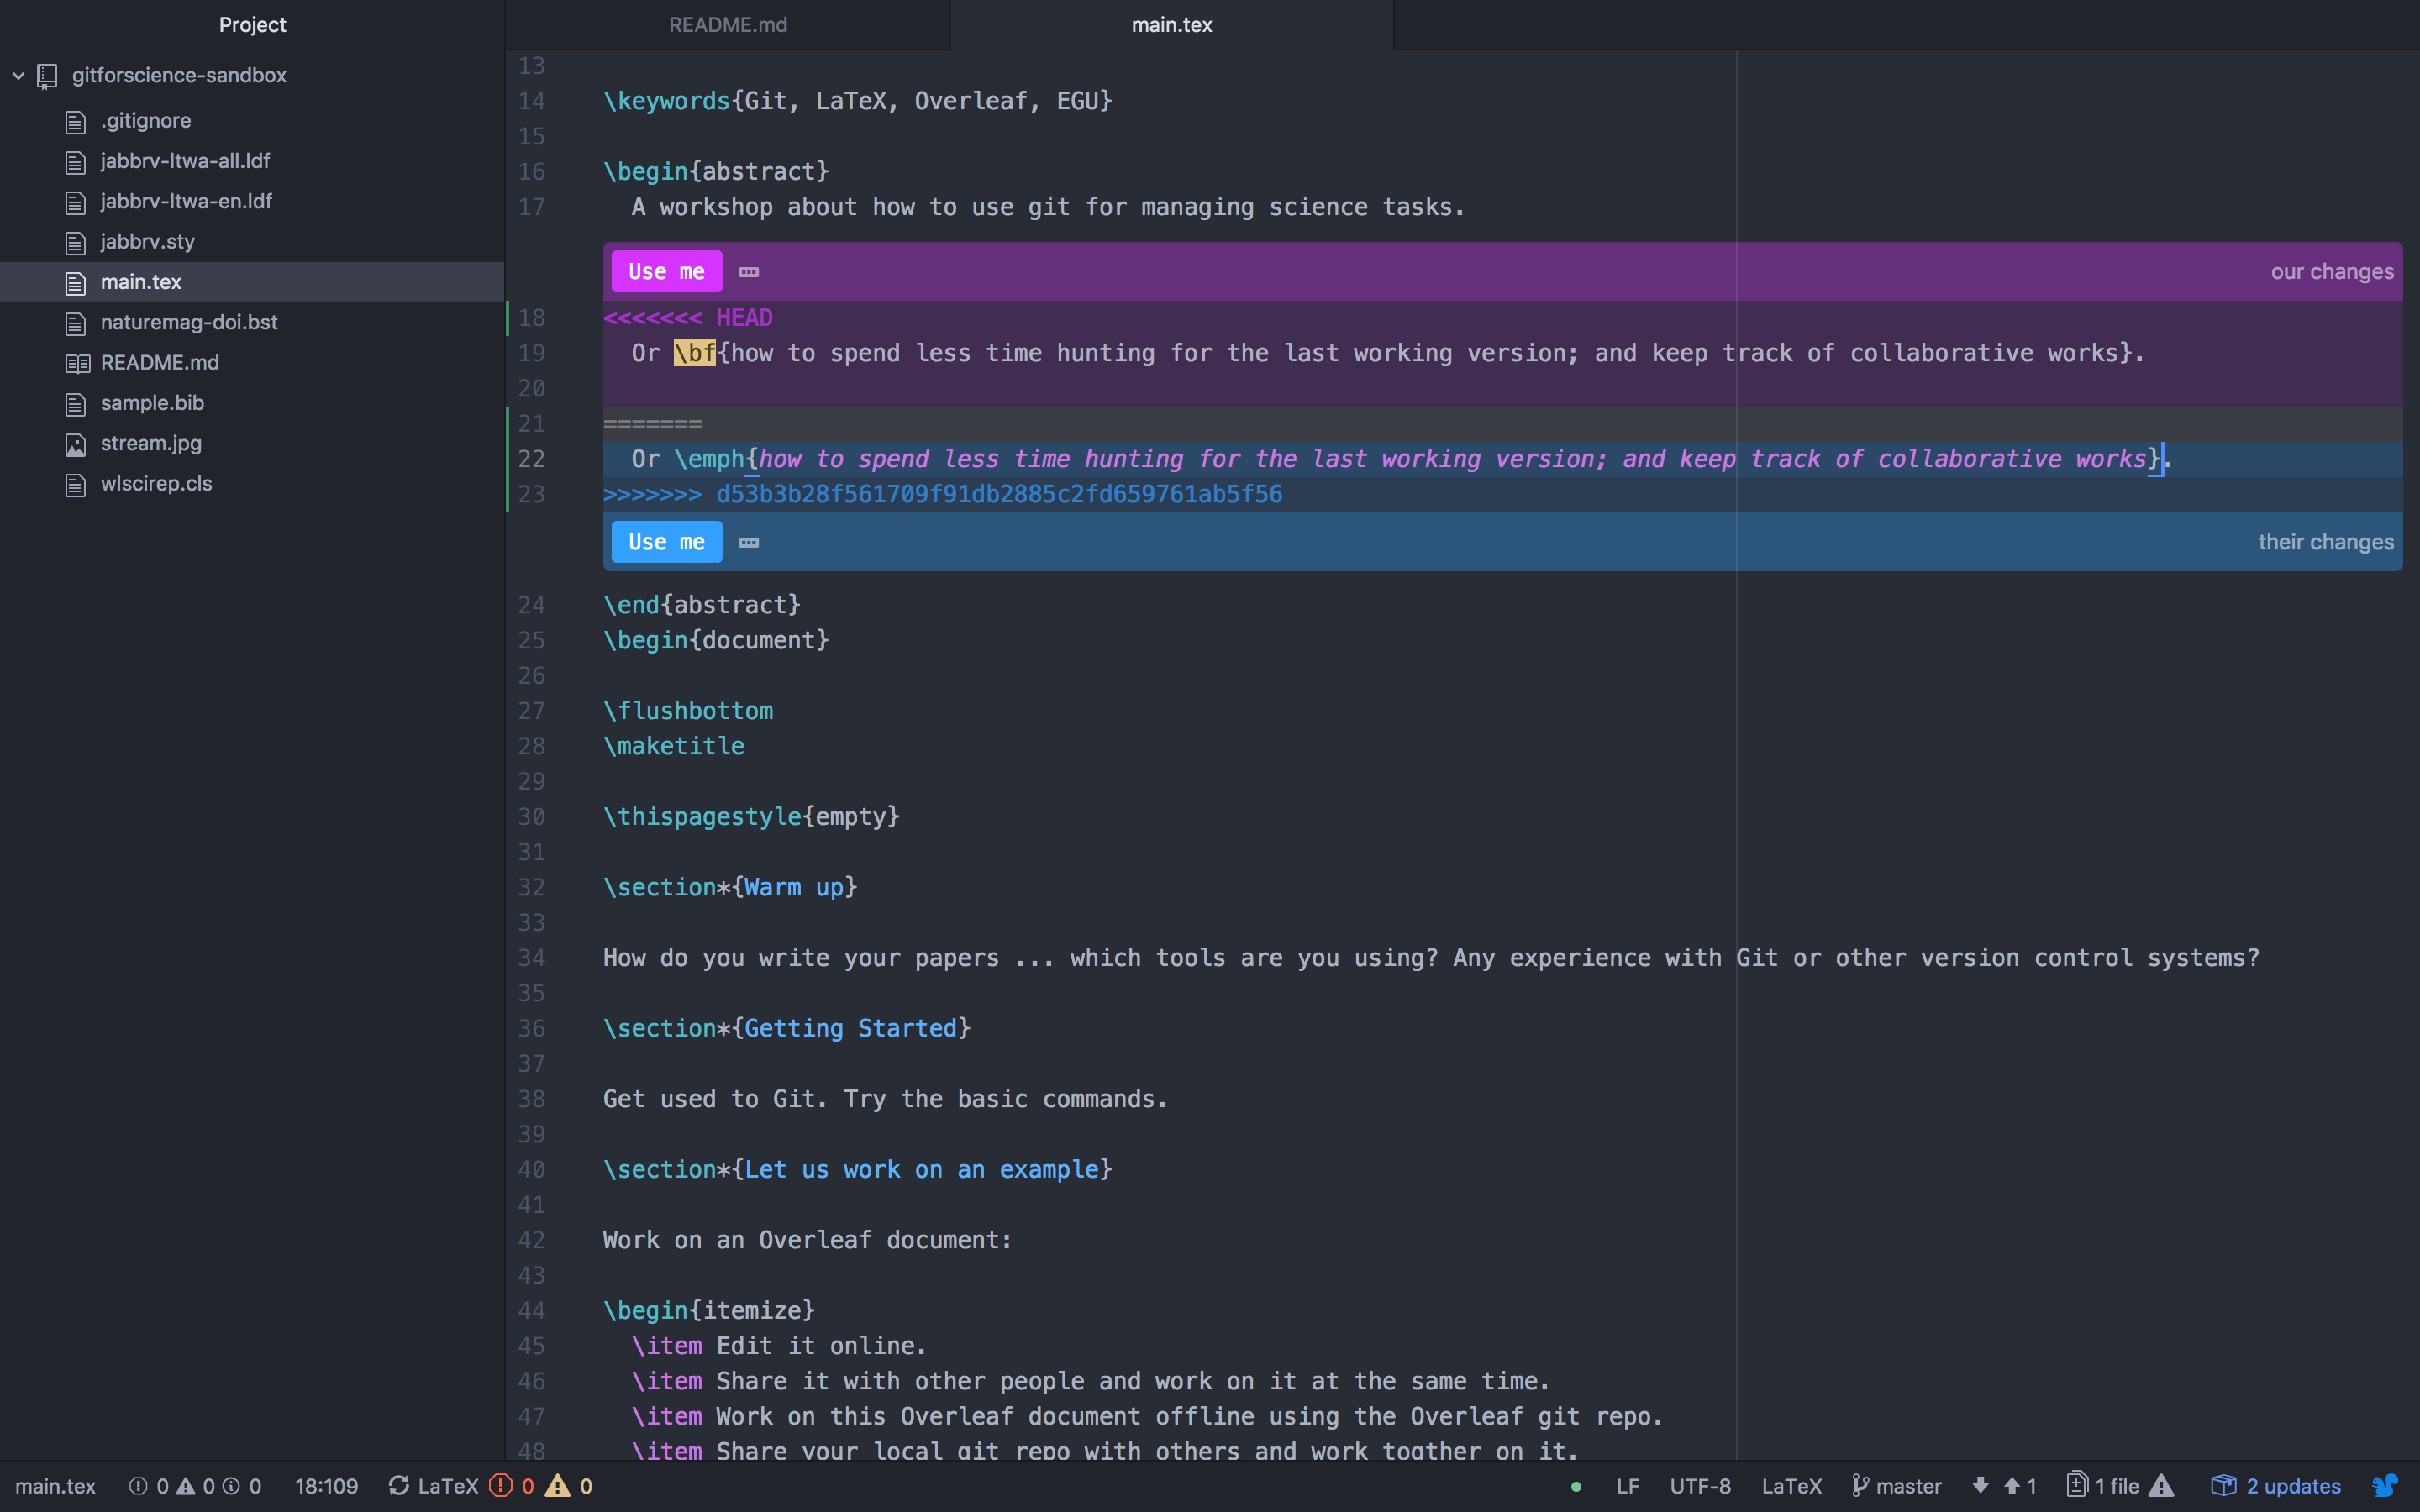
\includegraphics[width=20em]{atom-conflict}

\section*{Discussion}

Questions? Are these tools useful for you? Will you try them?

\end{document}
